% Included in tool.tex
\subsection{Direct Manipulation (DM) Gesture Set}

\begin{table}[!b]
% % increase table row spacing, adjust to taste
\renewcommand{\arraystretch}{1.75}
% if using array.sty, it might be a good idea to tweak the value of
% \extrarowheight as needed to properly center the text within the cells
% \setlength{\extrarowheight}{10pt}
\centering
% % Some packages, such as MDW tools, offer better commands for making tables %
% than the plain LaTeX2e tabular which is used here.
\begin{tabular}{|p{3.8cm} |p{3.8cm} |}
\hline
\textbf{Algorithm Behavior} & \textbf{DM Gesture} \\
\hline
%Access a value & Grab value and drag elsewhere \\
%\hline
Use or copy an object's value & {\em drag-away}: Grab an object, and drag it
away quickly.
Drop it on the stage to create a new number with the same value.
\\
\hline
Remove an object from its parent (e.g. element from list, node from tree/graph) & {\em dwell-drag-away}: Grab an object, dwell for one second, then
drag it elsewhere.
\\
\hline
Compare two objects' values & {\em drag-into}: Drag one value into another.
\\
\hline
Assign one object's value to another &
{\em drag-into-dwell}: Drag one value into another, and
dwell until the desired interpretation (\texttt{=, +=, -=}) appears. \\
\hline
Insert a value into a list, or a node into a tree/graph
& {\em drag-insert}: Drag the value into a gap in the list, or the node to the
tip of an edge
\\

\hline
Attach an edge to a graph node
& {\em drag-edge}: Drag the edge's start or end handle to the node.
\\

\hline
Mark a list element or tree/graph node (e.g. as sorted or visited) &
{\em fill}: Select the ``Fill" tool, and click on the element. \\
\hline
\end{tabular}

\caption{CodeInk's Direct Manipulation (DM) Gesture Set}
\label{tbl:gesture_table}

\end{table}

CodeInk's DM gesture set (summarized in \tab{tbl:gesture_table}) enables
users to trace algorithms by manipulating numbers, lists, binary trees and
graphs. From our experience of watching online lecture videos of an introductory
algorithms class, we compiled a list of algorithm behaviors that need to be
expressed when tracing commonly taught sorting and search algorithms (left
column of \tab{tbl:gesture_table}).
For each behavior, we then devised a gesture, in keeping with principles of direct
manipulation~\cite{Shneiderman1982, Lee2012}, that would enable the user to
express each behavior using a physical action. For example, numbers can be
copied by grabbing them and dragging away, and they can be inserted into lists
by dragging them into gaps between other elements.

All data structures in CodeInk's visual vocabulary are composed of one
or more objects (list elements or nodes), each with numeric values. For
that reason, the gesture set is both compact (7 gestures in total) and
expressive: dragging one object into another compares their numeric
values, regardless of whether they are numbers, list elements, nodes or
some mixture thereof. Similarly, popping a list element or detaching a
subtree from its parent is accomplished by grabbing and holding it
(\emph{dwelling}) until it can be moved away freely. We explain the
design decision behind dwelling later in this section. We now illustrate
the gesture set through two examples.

\noindent \textbf{Insertion Sort}: An instructor or student typically
traces insertion sort on an example list by redrawing it in successive
configurations (\fig{fig:6006-insertion}). With CodeInk, the algorithm
can be traced as follows:

\noindent 1) Drag an example list onto the stage (main canvas) and enter
numbers to initialize element values. Drag a finger onto the stage to
point to the starting element. The green arrows below indicate user drag
motion and are not part of the CodeInk UI.

\vspace{-0.25em}
\noindent 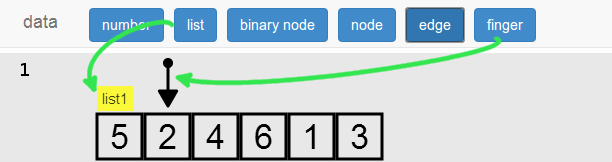
\includegraphics[width=0.7\columnwidth]{img/examples/insertion-1.png}
\vspace{0.5em}

\noindent 2) To prepare to move the ``2" element, grab and hold the element for
at least one second (\emph{dwell}). A blue circle fills up to give the user
feedback on how long they have dwelled.

\vspace{-0.25em}
\noindent 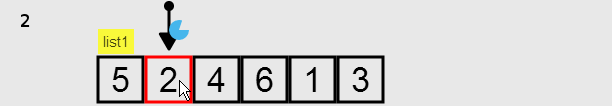
\includegraphics[width=0.7\columnwidth]{img/examples/insertion-2.png}
\vspace{0.4em}

\noindent 3) After one second has elapsed (blue circle filled entirely), the
list expands outward, creating gaps into which the element can be inserted. The
``2" element is now ready to be moved.

\vspace{-0.25em}
\noindent 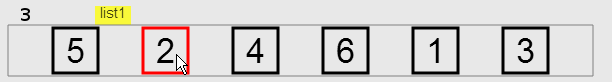
\includegraphics[width=0.7\columnwidth]{img/examples/insertion-3.png}
\vspace{0.5em}

\noindent 4) Drag the ``2" to the left until it hits the ``5" element, which
adds a numeric comparison step (``2 $<$ 5") to the trace.

\vspace{-0.25em}
\noindent 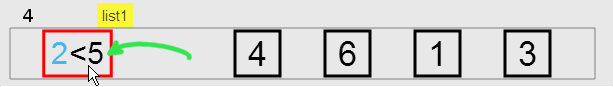
\includegraphics[width=0.7\columnwidth]{img/examples/insertion-4.png}
\vspace{0.5em}

\noindent 5) Keep moving the ``2" to the left of the ``5" element.

\vspace{-0.25em}
\noindent 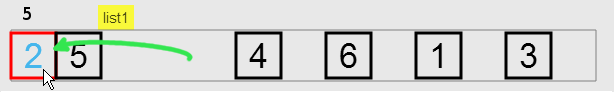
\includegraphics[width=0.7\columnwidth]{img/examples/insertion-5.png}
\vspace{0.5em}

\noindent 6) Once the correct position is found, drop the element
to adds a list insertion step to the trace. The list collapses again in its new, rearranged state, with the
``2" preceeding the ``5''.

\noindent 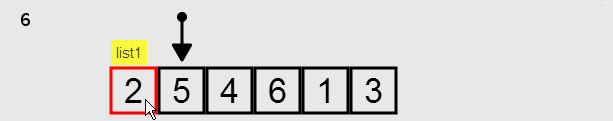
\includegraphics[width=0.7\columnwidth]{img/examples/insertion-6.png}

The user traces the rest of insertion sort by moving the finger down the
list and inserting elements into the sorted sublist until the entire
list is sorted. If any mistakes are made, the user can undo steps to
remove them from the trace.


\noindent \textbf{AVL Insertion}: Drawing an AVL (balanced binary search
tree) insertion can be tedious and error-prone, because rotations
require redrawing the entire tree in a new configuration. CodeInk's
gesture set affords users the ability to rearrange nodes in the tree by
detaching, dragging, and reattaching them. As is the case with lists,
dragging one value into another triggers a numeric comparison (Step 2),
and grabbing and dwelling removes a child from its parent (Step 5).


\noindent \begin{tabular}{m{4.6cm} m{3.4cm}}

1) Create two new binary tree nodes (``4" and ``6") by dragging node
objects onto the stage and typing in their numeric values.

& 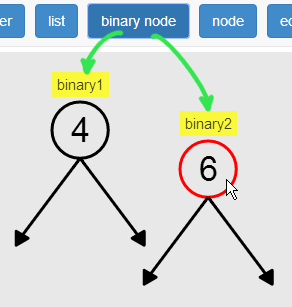
\includegraphics[width=3.4cm]{img/examples/bst-1.png}
\end{tabular}


\noindent \begin{tabular}{m{4.6cm} m{3.4cm}}

2) Drag the ``6'' node into the ``4'' node to compare their values.
CodeInk adds the comparison step (``4 $<$ 6") to the trace.

& 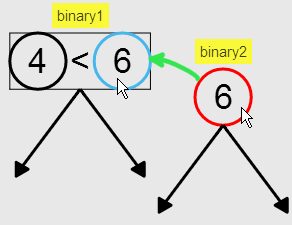
\includegraphics[width=3.4cm]{img/examples/bst-2.png}
\end{tabular}

\noindent \begin{tabular}{m{6.2cm} m{1.8cm}}

3) Since ``6" is greater than ``4", keep dragging the ``6'' along the
right pointer of the ``4" node. This gesture temporarily highlights the pointer
blue and adds a \emph{pointer traversal} step to the trace.

& 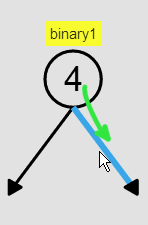
\includegraphics[width=1.8cm]{img/examples/bst-3.png}
\end{tabular}

\noindent \begin{tabular}{m{4.6cm} m{3.4cm}}

4) Keep dragging along the right pointer until reaching its tip. The
``6" node now re-emerges as the right child of ``4." The node is colored blue to
preview the insertion. Release the node to confirm the insertion and
add the step \texttt{binary1.right = binary2} to the trace.

& 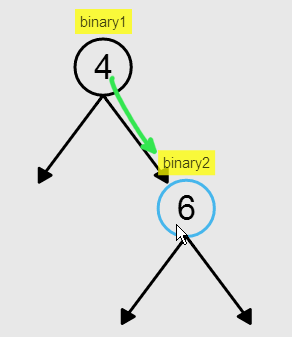
\includegraphics[width=3.4cm]{img/examples/bst-4.png}
\end{tabular}

\noindent \begin{tabular}{m{4.6cm} m{3.4cm}}

5) Next insert a new ``9" node into the tree, which results in an
unbalanced tree. Now demonstrate a rotation by grabbing the ``6" node,
dwelling for one second, and dragging it away to detach the subtree.
When the subtree is dropped on the stage, a new step is added to the
trace: \texttt{binary1.right = None}

& 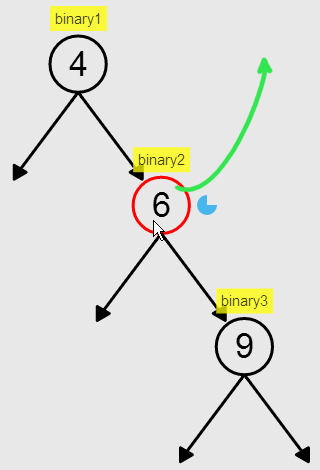
\includegraphics[width=3.4cm]{img/examples/bst-5.png}
\end{tabular}

\noindent \begin{tabular}{m{4.6cm} m{3.4cm}}

6) The ``6 / 9" subtree is now separated from the ``4." Drag the ``4"
node downward ...

& 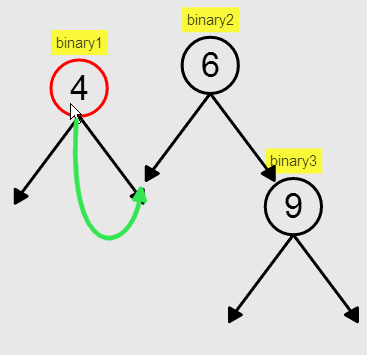
\includegraphics[width=3.4cm]{img/examples/bst-6.png}
\end{tabular}

\noindent \begin{tabular}{m{4.6cm} m{3.4cm}}

7) ... until it reaches the tip of the ``6" node's left pointer. Then
release to insert it there and balance the tree, thereby adding the step
\texttt{binary2.left = binary1} to the trace.

& 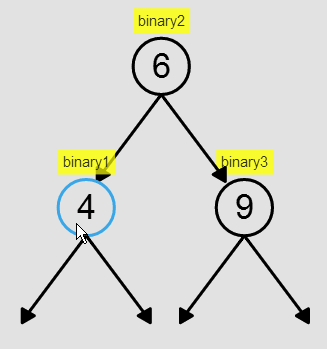
\includegraphics[width=3.4cm]{img/examples/bst-7.png}
\end{tabular}

\begin{comment}
\noindent \textbf{Graph algorithms}: Our gesture set also covers graph
traversal, such as search or finding shortest paths (see
\fig{fig:example-dijkstra}). It supports creating and attaching graph
nodes and edges, updating node and edge values, and marking nodes as
visited. Here is how to trace Dijkstra's algorithm using CodeInk:

\noindent \begin{tabular}{m{4.2cm} m{3.8cm}}
1) Create an example graph by dragging and dropping node and edge
objects onto the stage, typing in the numeric node costs and edge weights.
Edges can be connected to nodes by clicking and dragging their start and end
handles.
& 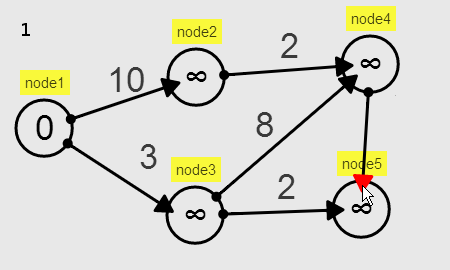
\includegraphics[width=3.8cm]{img/examples/dijkstra-1.png}
\end{tabular}

\noindent \begin{tabular}{m{4.2cm} m{3.8cm}}
2) Start with \texttt{node1}. To calculate the
cost of reaching its neighbor \texttt{node2},
first drag \texttt{node1} (source node) and drop it onto the stage, which
creates a new number (\texttt{num1}) equal to the node's cost (\texttt{0}).
& 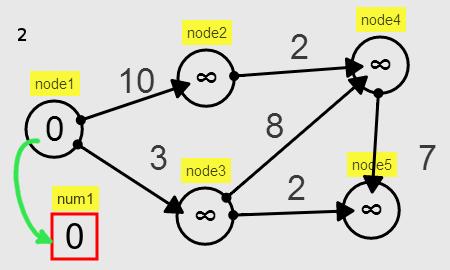
\includegraphics[width=3.8cm]{img/examples/dijkstra-2.png}
\end{tabular}

\noindent \begin{tabular}{m{4.2cm} m{3.8cm}}
3) Now drag the weight of the connecting edge into the current cost
(\texttt{num1}), which triggers a comparison by default. However, a
comparison is not the correct operation; the two values
must be added.
& 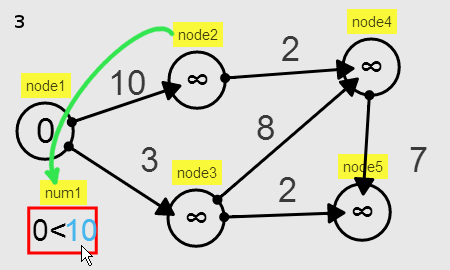
\includegraphics[width=3.8cm]{img/examples/dijkstra-3.png}
\end{tabular}

\noindent \begin{tabular}{m{4.2cm} m{3.8cm}}
4) Dwelling after the drag-into gesture causes CodeInk to cycle through alternative
interpretations. When an addition assignment
operation (\texttt{+=}) appears, release to end the gesture. The cost
updates to the value of \texttt{10} (\texttt{num1 += edge1.weight}).
& 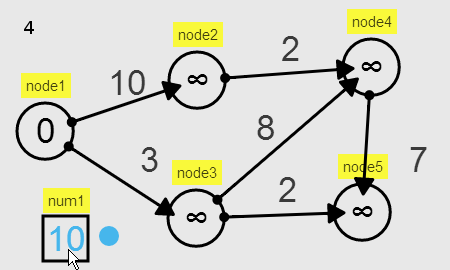
\includegraphics[width=3.8cm]{img/examples/dijkstra-4.png}
\end{tabular}

\noindent \begin{tabular}{m{4.2cm} m{3.8cm}}
5) Now drag \texttt{num1} into \texttt{node2}
to trigger a comparison, checking if the new cost is less than
the existing cost of reaching that node.
& 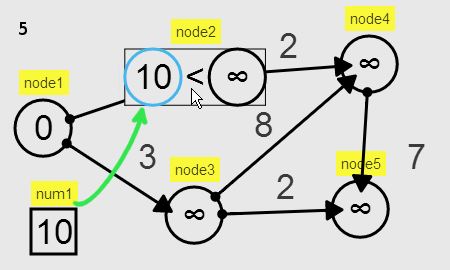
\includegraphics[width=3.8cm]{img/examples/dijkstra-5.png}
\end{tabular}

\noindent \begin{tabular}{m{4.2cm} m{3.8cm}}
6) Since \texttt{10 $<$ $\infty$}, dwell to cycle to the assignment
expression (\texttt{node2.value = num1}). Releasing ends the gesture, and updates the cost
of \texttt{node2} to 10.
& 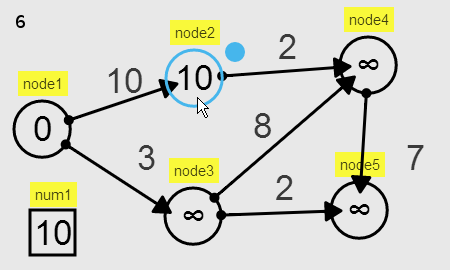
\includegraphics[width=3.8cm]{img/examples/dijkstra-6.png}
\end{tabular}

\noindent \begin{tabular}{m{4.2cm} m{3.8cm}}
7) Repeat on all nodes and mark each one as visited by
selecting ``Fill" and clicking on that node.
& 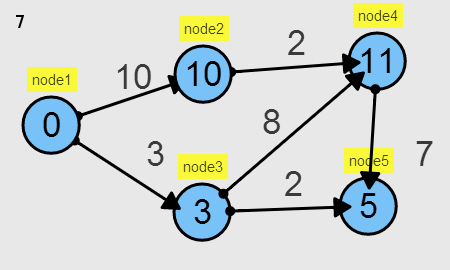
\includegraphics[width=3.8cm]{img/examples/dijkstra-7.png}
\end{tabular}

%Because the drag-into gesture has multiple interpretations
%(comparison, assignment, addition assignment), the user can dwell
%to cycle through all interpretations (see \sec{sec:overloaded-gestures}).
\end{comment}

\subsection{Chaining and traversal patterns}
In CodeInk, the user can chain multiple gestures while dragging an object to
describe a traversal pattern. For example, during insertion sort, the user can
drag an element along the list, performing comparisons without releasing it
until the correct location is found. Similarly, during an AVL insertion, a
candidate node is dragged through the tree to make comparisons and follow
pointers to find the insertion point.

One subtle interaction issue is deciding which behaviors in a chain of
gestures to commit (add) to the trace. For example, the user should be
allowed to click and drag an element into a list, then undo the behavior
by dragging it back out before releasing the mouse button. The insertion
step should be committed only if the new value is released into the
list, but comparisons should be committed as the user is dragging the
element as part of a traversal pattern. We therefore distinguish between
\emph{mutation} and \emph{observation} behaviors as those that affect
the underlying data and those that only visualize decision making in the
algorithm, respectively. In a chain of gestures, observation behaviors
(e.g., comparisons) are continuously committed to the trace, while
mutation behaviors (e.g., insertions) are committed only at the end of a
gesture.

\subsection{Resolving overloaded gestures}
\label{sec:overloaded-gestures}

% When designing a gesture vocabulary, the gesture that seems most
% natural for a task can often be interpreted in multiple ways.
\tab{tbl:gesture_table} shows two overloaded gestures: drag-into and
drag-away. Drag-into is ambiguous because dragging one object into
another could be interpreted as a comparison (\texttt{x$<$y}) or an
assignment (\texttt{x=y}).
% or an augmented assignment such as \texttt{x+=y} or \texttt{x-=y}.
Performing the drag-away gesture on a child object is ambiguous because
it is not obvious whether the parent object should be altered. For
example, when dragging an element away from a list, should a copy of the
element be made, or should the element be popped from the parent list?
% For trees and graphs, should a copy of the dragged node be made, or
% should that node and its descendants be detached from the parent?
%
Our solution defaults to safe observation behaviors and previews other
possible mutation behaviors if the user dwells -- grabs and holds the
object -- for more than one second.
% This means defaulting to a comparison for the drag-into gesture, and
% making a copy of the dragged value for the drag-away gesture.
This design also aligns well with chained traversal patterns, since
comparisons can occur in quick succession while dragging.

